\documentclass[11pt,letterpaper]{article}
\usepackage{pslatex}
\usepackage[spanish]{babel}
\usepackage[utf8]{inputenc} % Caracteres con acentos.
\usepackage{latexsym}
\usepackage{amssymb} 
\usepackage{amsmath}
\usepackage{epsfig}
\usepackage{url}
\usepackage{natbib}
\usepackage{graphicx}
\graphicspath{ {imagenes/} }

\begin{document}

\pagestyle{empty}

\title{
Sistema de riego inteligente\\
}
\author{
Nicolás Gastón Maturana Barrios\\
Benjamin Ingram\\
Carrera de Ingeniería Civil en Computación\\ 
Universidad de Talca}
\date{\today}

\maketitle


\section{Descripción de la propuesta}

\subsection{Contexto del proyecto}
El proyecto consiste en desarrollar un sistema de riego autónomo e inteligente ideal para las personas que viajan mucho y les gusta mantener sus jardines en buen estado. Lo que se busca es reducir la intervención humana, aumentar la eficiencia en el uso del agua, ahorrar dinero y entregar datos estadísticos a los usuarios. El sistema básicamente cociste en sensores de humedad del suelo, un microcomputador y válvulas. Cuando un sensor detecte que la humedad del suelo no es la adecuada para mantener el jardín en buen estado, le envía una señal a la raspberry la que a su vez analiza datos meteorológicos y decide si es necesario o no hacer un riego. Con todo esto, se asegura que el jardín se encuentre en buen estado utilizando la menor cantidad de agua posible.\\
Para el proyecto se utiliza un microcomputador el cual se programa en Python, y es el encargado de recibir los datos de entradas, que en este caso son los datos meteorológicos y los del sensor de humedad. Una vez que los datos son recibidos el microcomputador los analiza y si se requiere un riego envía una señal la válvula solenoide que permitirá el paso del agua. También se utilizará un sensor de flujo para medir la cantidad de agua que se esta utilizando y así entregar reportes al usuario.\\
Cabe destacar que este sistema no solo es útil para los jardines, sino que también se puede utilizar para los huertos y/o predios agrícolas que utilizan sistemas de riego automáticos.

\newpage

\subsection{Trabajo relacionado} 
Los trabajos que hoy en día son utilizados para resolver este problema cumplen su propósito general, que es el de automatizar el riego, pero en esta solución aun se requiere la intervención de las personas para su funcionamiento, como lo son los sistemas que utilizan temporizadores \citep{temporizador}. Estos trabajos utilizan temporizadores que se activan cada cierto intervalo de tiempo sin tomar en cuenta variables importantes como lo son la humedad del suelo. También existen trabajos en los que se mide la humedad del suelo \citep{temporizadorSensorHumedad} pero aun no se logra darle al agua de riego el uso óptimo, ya que no toma en cuenta los datos meteorológicos y en caso que se aproxime una lluvia el sistema igual hará el riego.\\
En el mercado tenemos la opción de automatizar nuestro riego pero son opciones que tienen un costo muy elevado, estas soluciones las podemos encontrar en las tiendas de retail.\\
Por otro lado tampoco indican el consumo de agua que se ha utilizado en el riego y tampoco tienen sistema de prevención en caso de condiciones climáticas extremas, como puede ser el frío extremo que nos ayuden a mantener en buen estado nuestro jardín.


\subsection{Definición del problema} 
A muchas personas les gusta mantener un jardín verde, pero generalmente no tienen el tiempo para regar y mantener su jardín como les gustaría. Por otro lado tenemos todos los problemas que genera el cambio climático, como lo son las temperaturas extremas y siendo uno de los principales afectados los recursos hídricos \citep{cambioClimatico}. Con la implementación de este proyecto, se busca que la mantención del jardín de un hogar sea de una forma autónoma e inteligente, es decir, que no necesite la intervención de personas para su funcionamiento y que en lo posible no utilice mas agua de la debida.\\
Otro problema es el causado por las temperaturas extremas, que pueden producir mucho daño en el jardín, llegando a extremos en el que se pierde todo. Pero ¿Cuanto agua he utilizado? ¿Cuanto dinero  he gastado en el agua para riego? ¿Cuantos riego ha tenido mi jardín? son preguntas que las personas se hacen y no tienen respuesta.

\newpage

\subsection{Propuesta de solución}
Como solución al problema, se creara un prototipo de riego automático e inteligente. Esto se hará utilizando un microcomputador y sensores de humedad. Lo distinto que tendrá este sistema de otros, es que para determinar si se debe hacer un riego o no, tomará en cuenta datos meteorológicos obtenidos desde internet, y en caso de que se pronostique una lluvia, no se hará el riego. El sistema contara con un GPS para determinar la posición en la que se encuentra el jardín a regar y obtener los datos meteorológicos. También contará con un sistema preventivo que ayude al cuidado del jardín, por ejemplo cuando se detecte que habrá una helada y ésta puede producir algún tipo daño, el sistema podrá enviar un mensaje al usuario o podrá activar el sistema de riego para así prevenir daños.\\
El sistema almacenará toda la información recopilada por los sensores guardándola en un único servidor, con lo que los usuarios utilizando un usuario y una contraseña podrán consultar los datos estadísticos a través de una aplicación web o una móvil. Este servidor que tendrá la base de datos, también será utilizado en caso que de el microcomputador deje de funcionar, ya que éste estará constante mente enviando una señal al servidor para saber si el sistema esta funcionando o no, para así informar a los usuarios de que el sistema esta fallando, asegurando un funcionamiento a lo largo del tiempo.\\
Con toda la información que el sistema recibe como entrada, será utilizada para generar un modelo de riego con el que se espera darle una mayor eficiencia al agua que es utilizada en el riego.\\
Todo esto hará que el sistema sea inteligente al momento de generar un riego, sacando totalmente a las personas de esta tarea, además entregando información que le puede ser útil a los usuarios.

\newpage

\section{Hipótesis}
\begin{itemize}
\item El prototipo es realizable con la tecnología existente.
\item El uso de este sistema disminuirá el consumo de agua utilizado en el riego del jardín.
\item Las personas dejarán de preocuparse por el riego de su jardín.
\item El uso de este sistema cuidará el jardín en todas las estaciones del año.
\item La utilización del modelo de riego disminuirá el consumo de agua.
\end{itemize}

\section{Objetivos}
\paragraph{Objetivo general}
\begin{itemize}
\item El objetivo es automatizar el riego de un jardín utilizando un sistema inteligente.
\end{itemize}

\paragraph{Objetivos específicos}
\begin{itemize}
\item Generar un modelo de riego con los datos obtenidos.
\item Quitar la intervención humana en el riego del jardín.
\item Mantener a los usuarios informados con datos estadísticos.
\item Tener un sistema preventivo en caso de condiciones climáticas extremas o el sistema deje de funcionar.
\end{itemize}

\section{Alcances}
\begin{itemize}
\item En este trabajo se espera implementar un prototipo funcional de la idea a desarrollar.
\item Este trabajo se limita a el control del riego, el sistema de riego (cañerías, aspersores, etc.) deben estar instalados.
\item En los datos estadísticos, se espera entregar al usuario al menos el consumo de agua utilizado en el riego.
\end{itemize}

\newpage

\section{Metodología}

\paragraph{Objetivo 1:} ``Generar un modelo de riego con los datos obtenidos"\\
\begin{itemize}
\item Generar un modelo de riego con los datos de entradas disponibles.
\item Obtener datos de los sensores utilizando el microcomputador.
\item Obtener la posición geográfica utilizando el GPS.
\item Obtener datos climatológicos desde internet utilizando el microcomputador.
\item Hacer pruebas al modelo de riego generado.
\end{itemize}

\paragraph{Objetivo 2:} ``Quitar la intervención humana en el riego del jardín"\\
\begin{itemize}
\item Aprender a utilizar el microcomputador (RaspberryPi).
\item Estudiar Python.
\item Aprende a utilizar la interfaz GPIO de RaspberryPi.
\item Aprender a activar y desactivar una válvula solenoide desde el microcomputador.
\end{itemize}

\paragraph{Objetivo 3:} ``Mantener a los usuarios informados con datos estadísticos"\\
\begin{itemize}
\item Leer datos desde un sensor de flujo de agua.
\item Configurar base de datos para el sistema.
\item Establecer conexión entre el microcomputador y la base de datos.
\item Enviar datos a la base de datos.
\item Generar el gráfico.
\item Hacer una aplicación web o móvil que se conecte a la base de datos para que los usuarios consulten las estadísticos.
\end{itemize}

\paragraph{Objetivo 4:} ``Tener un sistema preventivo en caso de condiciones climáticas extremas"\\
\begin{itemize}
\item Analizar los datos meteorológicos.
\item Enviar notificaciones a los usuarios.
\end{itemize}


\section{Plan de trabajo}

\paragraph{Etapa 1:} Desarrollar el objetivo 2 (27/04-19/06)
\begin{itemize}
\item Aprender a utilizar microcomputador (27/04-08/05)
\item Estudiar Python (11/05-15/05)
\item Escribir contexto del proyecto (18/05-27/05)
\item Utilizar la interfaz GPIO (28/05-13/06)
\item Activar y desactivar una válvula solenoide (15/06-19/06)
\end{itemize}

\paragraph{Etapa 2:} Desarrollar el objetivo 1 (22/06-término)
\begin{itemize}
\item Entrega final del análisis del problema (22/06-01/07)
\item Entrega final del informa de memoria (13/07-22-07)
\item Generar un modelo de riego (02/07-21/08)
\item Obtener datos de los sensores (24/08-28/08)
\item Obtener la posición geográfica GPS (31/08-04/09)
\item Obtener datos climatológicos desde internet (07/09-11/09)
\item Hacer pruebas al modelo de riego generado (11/09-02/10)
\end{itemize}

\paragraph{Etapa 3:} Desarrollar el objetivo 4 (05/10-09/10)
\begin{itemize}
\item Analizar los datos meteorológicos (05/10-09/10)
\item Enviar notificaciones a los usuarios (05/10-09/10)
\end{itemize}

\paragraph{Etapa 4:} Desarrollar el objetivo 3 (12/10-30/10)
\begin{itemize}
\item Leer datos desde un sensor de flujo de agua (12/10-14/10)
\item Configurar base de datos (15/10-16/10)
\item Establecer conexión entre el microcomputador y la base de datos (15/10-16/10)
\item Enviar datos a la base de datos (15/10-16/10)
\item Generar el gráfico (19/10-21/10)
\item Hacer una aplicación web o móvil que se conecte a la base de datos para que los usuarios consulten las estadísticos. (19/10-30/10)
\end{itemize}

\newpage

%-------------------------------------------------------------------------------
%-------------------------------------------------------------------------------
%Marco Teórico

\section{Marco teórico}

%-------------------------------------------------------------------------------

\subsection{Programación del riego}

La programación del riego, es la planificación de cuándo y qué cantidad de agua aplicar con el fin de mantener el crecimiento saludable de las plantas durante la estación de crecimiento. Es una práctica de gestión diaria esencial.

El momento adecuado del riego es una decisión crucial para la aplicación: 
\begin{itemize}
\item Satisfacer las necesidades de agua del cultivo para evitar la pérdida de rendimiento debido a la escasez de agua.
\item Maximizar la eficiencia del uso del agua de riego y conservar los recursos hídricos locales.
\end{itemize}

Un riego eficaz sólo es posible con un seguimiento periódico de las condiciones del agua del suelo y el desarrollo de lo que se esta cuidando (campos de cultivos o jardines) y con la previsión de las futuras necesidades de agua. Retrasar el riego hasta provoca estrés, o aplicar muy poca agua puede resultar en una pérdida sustancial. La aplicación de mucha agua se traducirá en costes adicionales y agua desperdiciada.

Existen varias herramientas que están disponibles para ayudar a un administrador el riego: sondas de suelo, sensores de humedad del suelo, estaciones meteorológicas, etc.

Para la programación del riego se utilizarán sensores de humedad del suelo y datos obtenidos de alguna estación meteorológica que entregará la probabilidad de lluvia en el lugar, cuando sea posible y a causa de que existe probabilidad de lluvia, la cantidad de agua de riego aplicada debe ser algo menor que el déficit de agua en el suelo con el fin de proporcionar el resto con la lluvia que caerá en el lugar.

Ora variable que se tendrá en cuenta, es el tipo de suelo en el que se encuentra ubicado el sistema de riego, ya que permitirá saber la capacidad de absorción  que éste tiene, con el conocimiento de esta información se podrá saber cuándo comenzar un riego con el fin de utilizar el agua de forma eficiente.


\subsubsection{Textura del suelo}

La textura indica el contenido relativo de partículas de diferente tamaño, como la arena, el limo y la arcilla, en el suelo. La textura tiene que ver con la facilidad con que se puede trabajar el suelo, la cantidad de agua y aire que retiene y la velocidad con que el agua penetra en el suelo y lo atraviesa.

Para conocer la textura de una muestra de suelo\citep{sueloTextura}:
\begin{itemize}
\item Arcilloso: Se adhiere bastante, es fácilmente moldeable, las partículas no son visibles y la superficie brilla levemente.
\item Limoso: Se adhiere a los dedos, se moldea con dificultad, los dedos dan apariencia grasosa y las partículas son brillantes.
\item Arenoso: No se pega en los dedos, no se moldea como una masa y sus partículas individuales son visibles.
\end{itemize}

Cada uno de estos tipos de suelos presentan una propiedad llamada permeabilidad; que es la característica que tiene el suelo de transmitir el agua y el aire y es una de las cualidades más importantes que han de considerarse a la hora de realizar un riego. Mientras más permeable sea el suelo, mayor sera la filtración.

Por regla general, como se muestra en la Figura 1, mientras más fina sea la textura del suelo, más lenta sera la permeabilidad:

\begin{figure}[ht!]
\caption{Permeabilidad según textura del suelo}
\centering
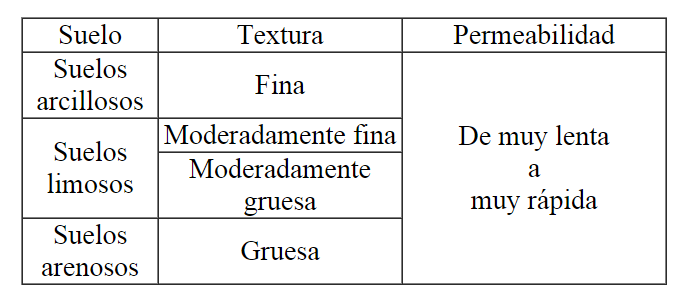
\includegraphics[width=7cm]{permeabilidad}
\end{figure}

%-------------------------------------------------------------------------------

\subsection{Servicios web meteorológicos}


\subsubsection{¿Qué es un servicio web?}

Los servicios web son sistemas de software que permiten el intercambio de datos y funcionalidad entre aplicaciones sobre una red. Esta soportado en diferentes 
estándares que garantizan la interoperabilidad de los servicios.\citep{webService}

En la Figura 1, se puede apreciar la arquitectura de un servicio web, se ve que el cliente realiza un petición al servidor y éste le envía una respuesta con lo solicitado.

\begin{figure}[ht!]
\caption{Arquitectura servicio web}
\centering
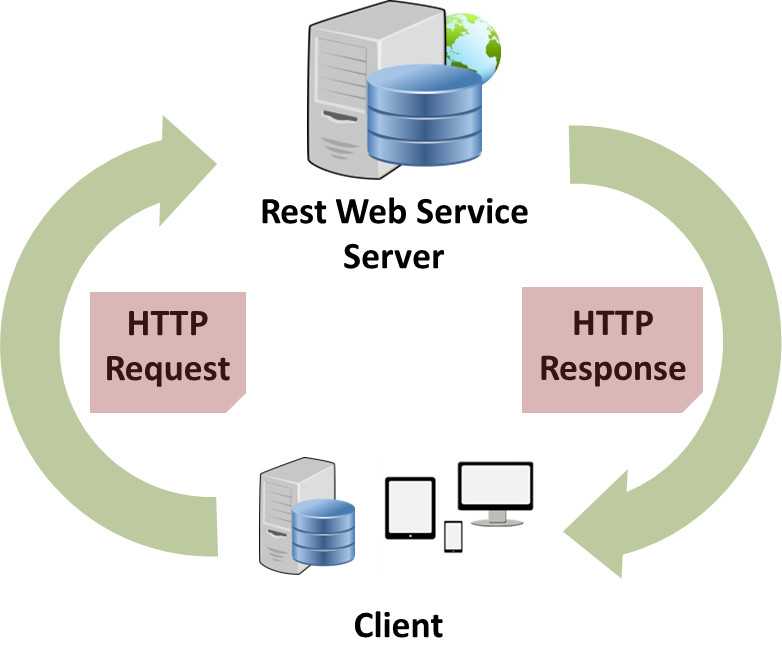
\includegraphics[width=7cm]{rest}
\end{figure}

Un servicio web REST, es un servicio implementado usando HTTP y que entrega como resultado un XML o un JSON de los cuales se puede obtener la información solicitada.


\subsubsection{Wunderground}

Weather Underground es un servicio que entrega información meteorológica que ha desafiado las convenciones en torno a cómo la información del tiempo se comparte con el público desde 1993. Se ha creado con el fin de mejorar el acceso de las personas a los datos meteorológicos significativos de todo el mundo. Como servicio meteorológico primero de Internet, son considerados pioneros en su campo y están en constante búsqueda de nuevos conjuntos de datos y tecnologías que ayuden a compartir más datos con más gente.

Wunderground no da la posibilidad de consultar el clima dado las coordenadas de la posición en la que un punto se encuentra, estas coordenadas pueden ser obtenidas de forma automática utilizando un GPS o ingresándolas manualmente. Para utilizar el servicio, es necesario registrarse para obtener un llave que se utiliza para realizar las consultas meteorológicas.

Para obtener más información y/o registrarse para utilizar el servicio se puede hacer en la siguiente url: 

\url{http://www.wunderground.com/weather/api/d/docs?d=index}\\

La estructura de la url para realizar la consulta de la siguiente:

\url{http://api.wunderground.com/api/e7d949410a7481dc/forecast10day/lang:SP/q/-34.40819094134256,-71.00087251514196.json}

\begin{itemize}
\item \url{http://api.wunderground.com/api/} es la dirección donde se hace la consulta.
\item \url{e7d949410a7481dc} es la llave que se obtiene al registrarse.
\item \url{forecast10day} retorna datos meteorológicos de los siguientes 10 días.
\item \url{lang:SP} se utiliza para obtener los datos en español.
\item \url{q/-34.40819094134256,-71.00087251514196} son las coordenadas del lugar que se quieren obtener los datos.
\item \url{.json} es el formato en el que se devuelve la información, también puede ser .xml.
\end{itemize}

Los datas obtenidos se pueden apreciar en la Figura 2:

\begin{figure}[ht]
\caption{Respuesta del servicio wunderground al hacer una consulta}
\centering
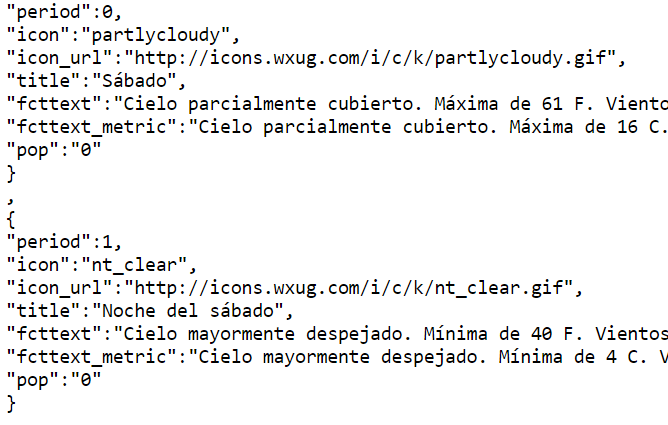
\includegraphics[width=13cm]{response}
\end{figure}

\newpage

De toda la información que entrega el servicio web wunderground, lo único que nos interesa hasta el momento, es el campo pop, que significa probabilidad de precipitación, que esta representada en porcentaje.


%-------------------------------------------------------------------------------

\subsection{Trabajos relacionados}

\subsubsection{Cultivar}

Cultivar está desarrollando y fabricando por Raincloud\citep{raincloud}. Raincloud administra de forma conveniente e inteligente la gestión del agua, con un sistema de riego conectado a la web que permite monitorear en todo momento es estado del sistema. Raincloud vincula los dispositivos móviles permitiendo activar válvulas de agua y consultar sensores de humedad utilizando Wi-Fi.\\

Ventajas:
\begin{itemize}
\item Utiliza sensores de humedad de suelo.
\item Se controla a través de un teléfono móvil.
\item Consume la menor cantidad de agua posible.
\item Almacena los datos en la nube.
\item Entrega estadísticas del consumo de agua.
\end{itemize}

Desventajas:
\begin{itemize}
\item Necesita configuración previa.
\item Se necesita Wi-Fi en el hogar para su óptimo funcionamiento.
\item Tiene un costo muy elevado. \$500 dolares.
\item No toma en cuenta datos meteorológicos.
\end{itemize}

\subsubsection{Rachio IRO}

Iro\citep{rachio} es un controlador de riego inteligente que permite a las personas de manera fácil, mantener sus jardines en buen estado. Se integra de manera fácil al Wi-Fi de su hogar, entregando un completo control a través de su computador o teléfono móvil.

Rachio se ajusta automáticamente a los datos meteorológicos del lugar en el que se encuentra, estación del año, tipo de zona y características de la región.\\

Ventajas:
\begin{itemize}
\item Se controla a través de un teléfono móvil o una computador.
\item Puede funcionar de forma automática. 
\item Se ajustara automáticamente a el clima.
\item Consume la menor cantidad de agua posible.
\item No necesita programarse.
\item Entrega estadísticas del consumo de agua.
\end{itemize}

Desventajas:
\begin{itemize}
\item No utiliza sensores de humedad de suelo.
\item Se necesita Wi-Fi en el hogar para su óptimo funcionamiento.
\item Tiene un costo muy elevado. \$249 / \$299 dolares.
\end{itemize}

%-------------------------------------------------------------------------------

\subsection{Hardware}

Todas las partes físicas de un sistema que tiene componentes: eléctricos, electrónicos, electromecánicos y mecánicos. Para la construcción del sistema de riego se necesitarán una serie de componentes, sensores, actuadores y computadores para su correcto funcionamiento.

\subsubsection{Raspberry pi}

El Raspberry Pi es un microcomputador del tamaño de una tarjeta de crédito a bajo costo que se conecta a un monitor o un televisor, utiliza un teclado y un ratón estándar. Es un dispositivo que permite a las personas de todas las edades explorar la computación y aprender a programar en lenguajes como Python. Es capaz de hacer todo lo que espera de una computadora de escritorio, desde navegar por Internet y reproducir vídeos en alta definición, trabajar en hojas de cálculo, procesadores de texto, y jugar juegos.

Raspberry Pi tiene la capacidad de interactuar con el mundo exterior, y se ha utilizado en una amplia gama de proyectos digitales, máquinas de música y detectores en las estaciones meteorológicas.\citep{raspberry}

\begin{figure}[ht!]
\caption{Raspberry Pi modelo B+}
\centering
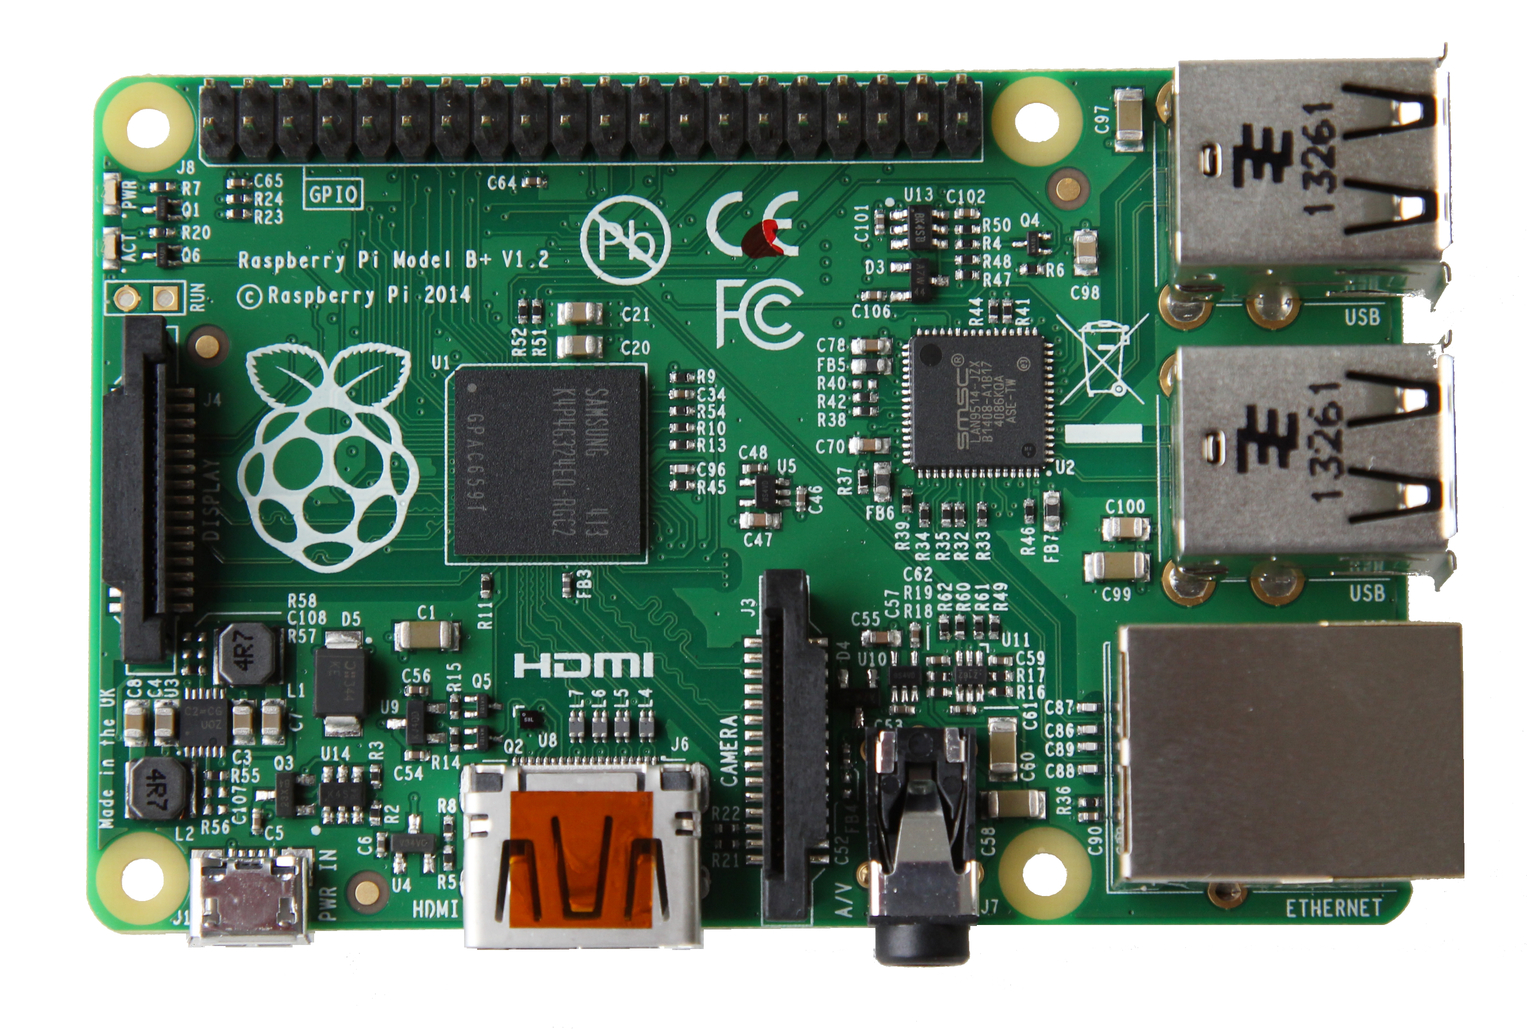
\includegraphics[width=5cm]{rasp}
\end{figure}

\newpage

\subsubsection{Comunicación serial}

La comunicación serial consiste en el envío de un bit de información de manera
secuencial, esto es, un bit a la vez y a un ritmo acordado entre el emisor y el receptor.
La Raspberry Pi cuenta con una interfaz de comunicación llamada GPIO que es utilizada para comunicarse con dispositivos externos.

\begin{figure}[ht!]
\caption{Comunicación serial entre la Raspberry Pi y una Protoboard}
\centering
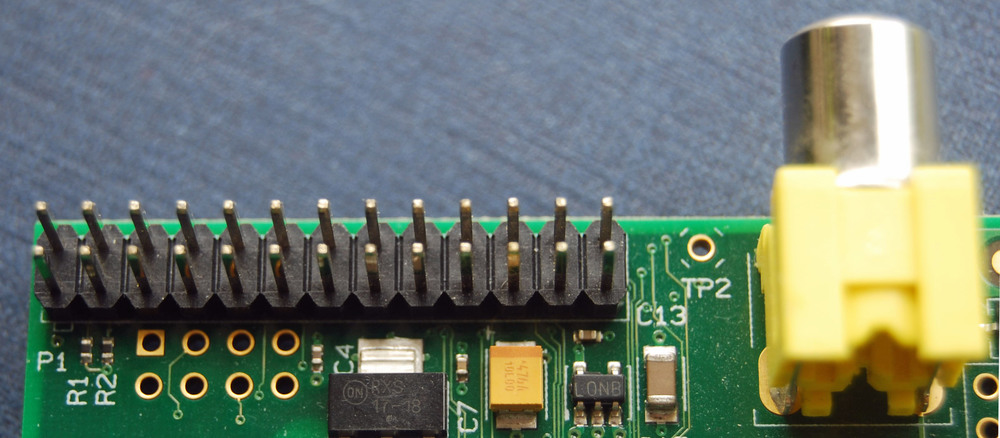
\includegraphics[width=5cm]{gpio}
\end{figure}

\subsubsection{Sensores de humedad}

Un sensor de resistencia eléctrica\citep{sensor}, estima indirectamente la tensión del suelo mediante la medición de la resistencia eléctrica utilizando alambre que va en un bloque de un material especial que mantiene su contenido de humedad en equilibrio con el suelo. La resistencia eléctrica dentro del bloque varía con el contenido de agua del suelo. 
Estos requieren poca preparación antes de la instalación y no requieren mantenimiento durante la temporada.

\begin{figure}[ht!]
\caption{Sensor de humedad}
\centering
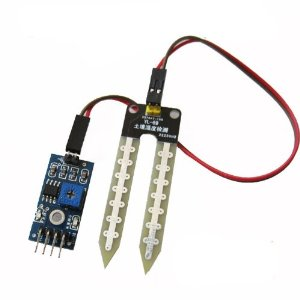
\includegraphics[width=5cm]{sensorHumedad}
\end{figure}

\newpage

\subsubsection{Sensor de flujo de agua}

El sensor de flujo de agua consiste en una válvula de cuerpo plástico, un rotor de agua y un sensor de efecto hall. Cuando el agua fluye a través del rotor, el rotor gira. Su velocidad cambia con diferentes ritmos de flujo. El sensor de efecto hall tiene como salida la señal de pulso correspondiente.

\begin{figure}[ht!]
\caption{Sensor de flujo de agua}
\centering
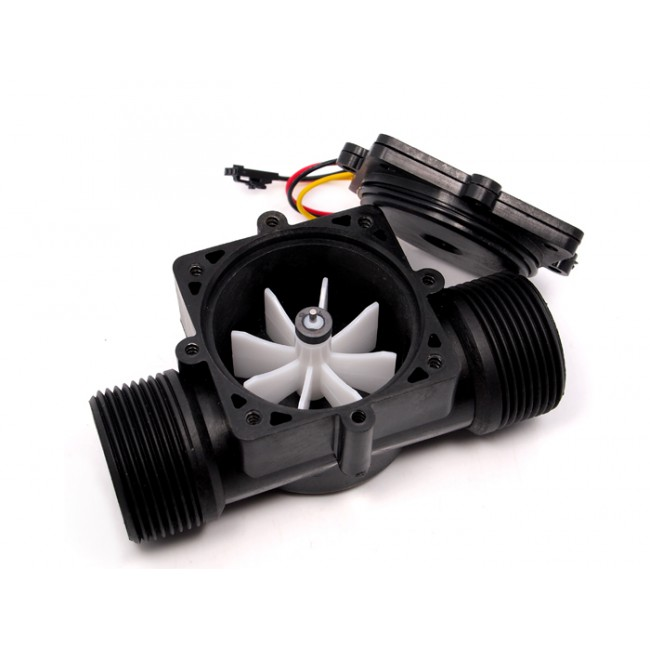
\includegraphics[width=5cm]{sensorFlujo}
\end{figure}

\subsubsection{Válvula solenoide}

Una válvula solenoide esta diseñada para controlar el paso de un fluido por un conducto o tubería. La válvula se mueve mediante una bobina solenoide. Generalmente no tiene más que dos posiciones: abierto y cerrado, o todo y nada. Las electroválvulas se usan en multitud de aplicaciones para controlar el flujo de todo tipo de fluidos.

\begin{figure}[ht!]
\caption{Válvula solenoide}
\centering
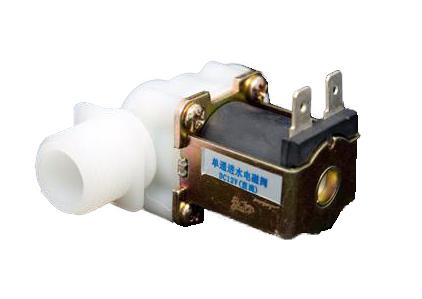
\includegraphics[width=5cm]{valvulasolenoide}
\end{figure}

\newpage

\subsubsection{GPS}

El sistema de posicionamiento global (GPS) es un sistema que permite determinar en todo el mundo la posición de un objeto y lo habitual son unos pocos metros de precisión.

\begin{figure}[ht!]
\caption{Módulo GPS USB}
\centering
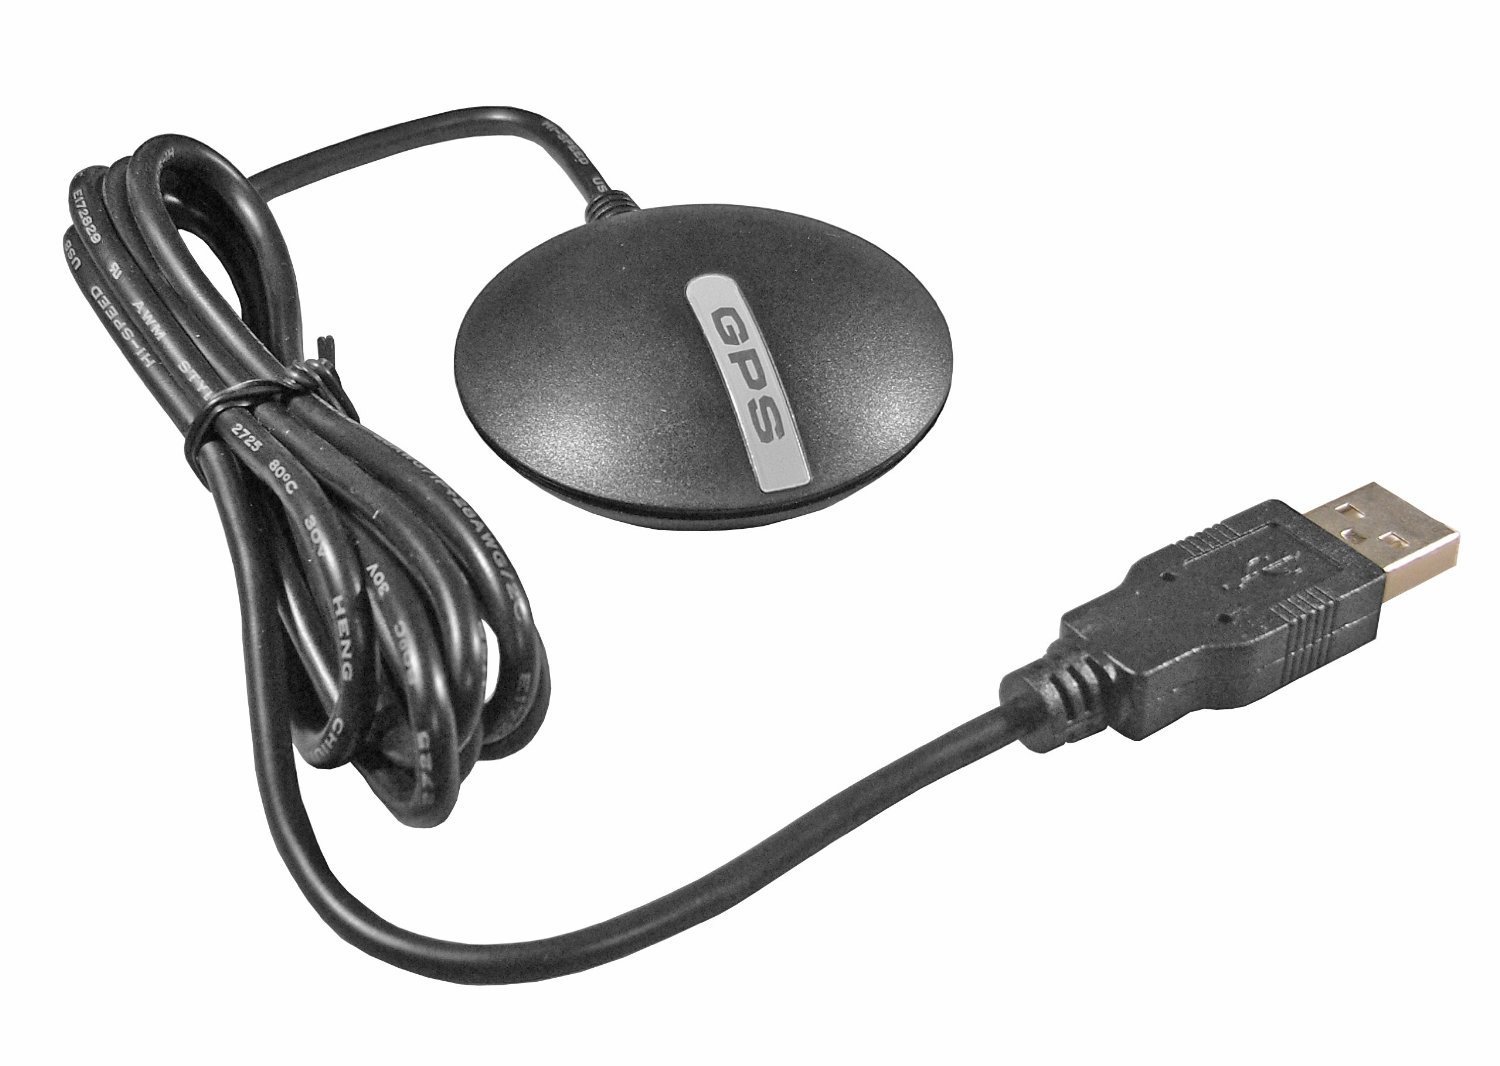
\includegraphics[width=5cm]{gps}
\end{figure}

\subsubsection{Módem 3G}

Módem 3G es un terminal de red inalámbrica basada en la tecnología CDMA2000. Es la mejor opción para los usuarios que necesiten acceder a Internet desde cualquier lugar en cualquier momento. El módem está conectado al microcomputador mediante una interfaz USB.

\begin{figure}[ht!]
\caption{Módem 3G}
\centering
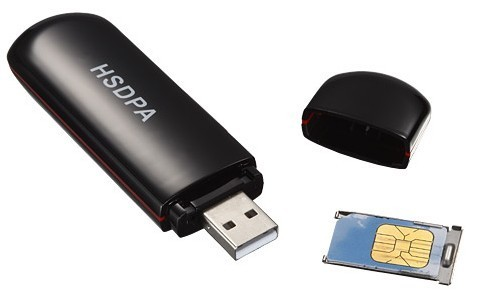
\includegraphics[width=5cm]{modem}
\end{figure}

\newpage

\subsubsection{Cargador}

Un cargador es un dispositivo utilizado para suministrar corriente eléctrica a un dispositivo, que en este caso se tratará de la Raspberry Pi. El cargador debe funcionar a 5V y entregar una corriente de 700mA.

\begin{figure}[ht!]
\caption{Cargador}
\centering
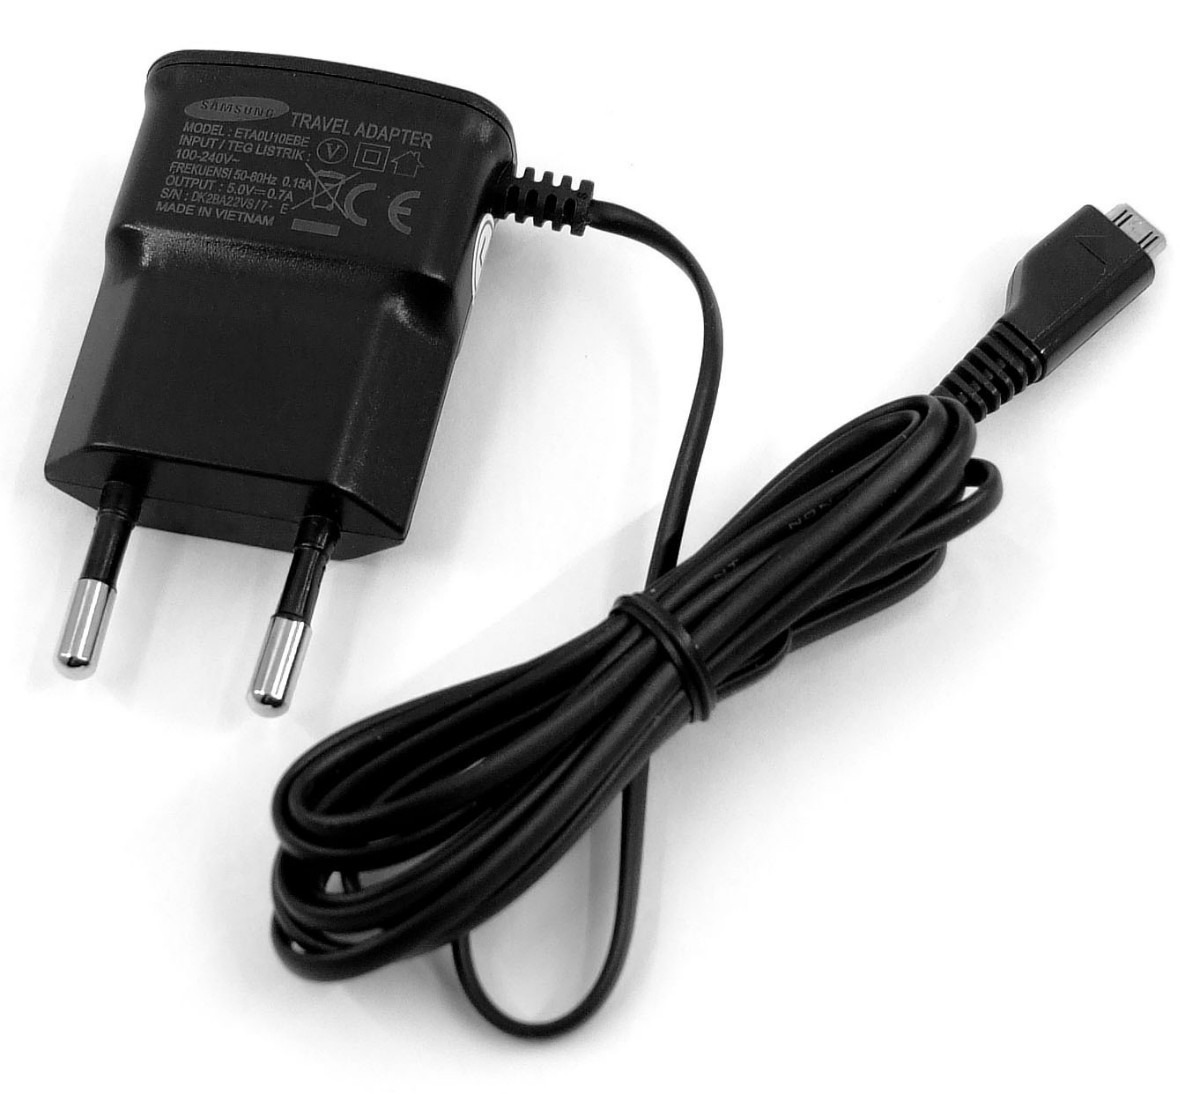
\includegraphics[width=5cm]{cargador}
\end{figure}

\newpage

%-------------------------------------------------------------------------------

\subsection{Software}

\subsubsection{Raspbian}

Raspbian\citep{raspbian} es un sistema operativo libre basado en Debían optimizado para el hardware Raspberry Pi. Un sistema operativo es el conjunto de programas básicos y utilidades que hacen que Raspberry Pi funcione. Sin embargo, Raspbian ofrece más que un sistema operativo; viene con más de 35.000 paquetes, software pre-compilado en un formato que hace más fácil la instalación en su Raspberry Pi.

Raspbian no tiene relación con la Fundación Raspberry Pi. Raspbian fue creado por un pequeño y dedicado equipo de desarrolladores que son fans del hardware Raspberry Pi.

Instalador: "\url{https://www.raspbian.org/RaspbianInstaller}"

\subsubsection{Python}

Python es un claro  y poderoso lenguaje de programación orientado a objetos, comparable con Perl, Ruby o Java.

Algunas de las caracteristicas de Python son:

\begin{itemize}
\item Python ideal para el desarrollo de prototipos y otras tareas de programación, sin comprometer la capacidad de mantenimiento.
\item Utiliza una sintaxis clara, por lo que los programas son fáciles de leer.
\item Viene con una biblioteca estándar que soporta muchas tareas comunes de programación, tales como la conexión a los servidores web, la búsqueda de texto con expresiones regulares, leer y modificar archivos.
\item Es software libre. No cuesta nada descargar o utilizar Python.
\item Tiene librerías que facilitan el uso de la interfaz GPIO de la Raspberry Pi.
\end{itemize}

https://wiki.python.org/moin/BeginnersGuide/Overview

\subsubsection{Librería GPIO}

Una de las características de gran alcance de la Raspberry Pi es la fila de GPIO\citep{gpio} (Entrada/Salida de Propósito General) alfileres a lo largo del borde de la placa, junto a la salida de vídeo socket amarilla como se puede apreciar en la Figura 11:

\begin{figure}[ht!]
\caption{GPIO Raspberry Pi}
\centering
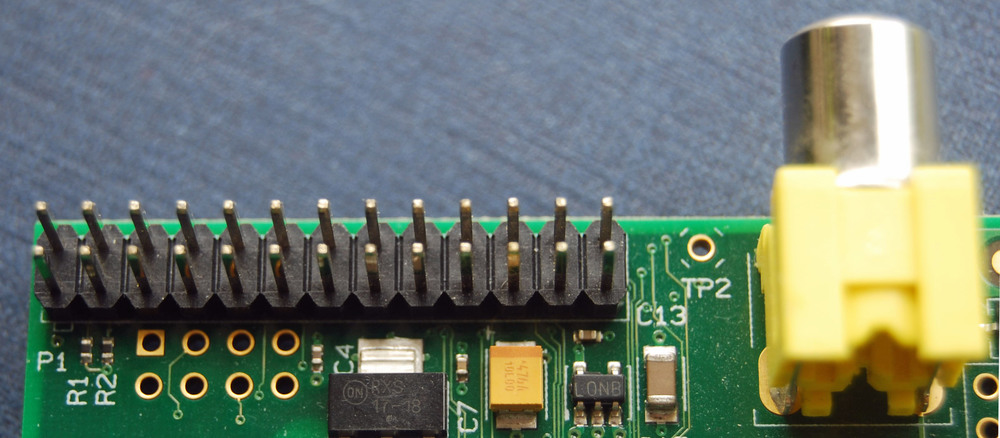
\includegraphics[width=7cm]{gpio}
\end{figure}

\newpage

Estos pines son una interfaz física entre el la Raspberry y el mundo exterior. Al nivel más simple, se puede pensar en ellos como interruptores que puede activar o desactivar ya sean las entradas como las salidas. Diecisiete de los veinte y seis pines son GPIO; los otros son pines de alimentación o de tierra como se ve en la Figura 12:

\begin{figure}[ht!]
\caption{Pines GPIO}
\centering
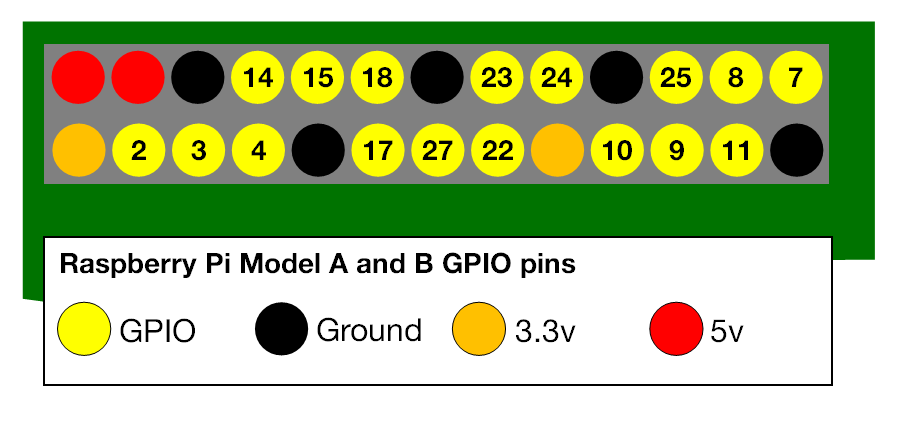
\includegraphics[width=7cm]{giop1}
\end{figure}

¿Qué puedo hacer con esto?\\

Puede programar los pines de maneras asombrosas para interactuar con el mundo real. Las entradas no tienen que venir de un interruptor físico; podría ser la entrada de un sensor o una señal de otro ordenador o dispositivo, por ejemplo. La salida también puede hacer cualquier cosa, desde encender un LED con el envío de una señal o de datos a otro dispositivo. Si la Raspberry está en una red, puede controlar los dispositivos que están conectados a él desde cualquier lugar. Conectividad y control de los dispositivos físicos a través de Internet es algo muy poderoso y emocionante, y la Raspberry es ideal para esto.
%-------------------------------------------------------------------------------

\newpage

\bibliographystyle{plain}
\bibliography{references}
\end{document}